
\section{Modelos com Desativação}

Abordaremos agora o modelo de reação-difusão com desativação de material
catalítico \cite{7}. O modelo trabalha sobre uma rede unidimensional de
sítios, onde cada sítio pode ser uma armadilha (um sítio catalítico) ou um sítio
inativo (material suporte).

Os sítios não se movem na rede durante a dinâmica e
as armadilhas (material catalítico) são distribuídas aleatoriamente com
recobrimento $\sigma_0$, enquanto os reagentes são distribuidos aleatoriamente
sobre os sítios inativos com recobrimento $\theta_0$. A distribuição de
reagentes e armadilhas respeita o vínculo $\sigma_0 + \theta_0 \leq 1$ e ela é
realizada antes de simularmos processo modelado. Não há fluxo de reagentes ou
reposição de armadilhas no decorrer da dinâmica.

A dinâmica do modelo se dá através da difusão de reagentes, que, ao se depararem
com um sítio ativo, reagem e saem instantaneamente do sistema, na forma de
produto.

O coeficiente de difusão é dado por $\mathcal{D}$, cujo valor expressa
o número de tentativas de se executar um passo do tamanho da rede, por unidade
de tempo, para cada reagente. A dinâmica de difusão respeita ainda o princípio
de volume excluído entre reagentes, de forma que um reagente tem execução de um
passo rejeitada quando a intenção do passo tem como alvo um sítio ocupado por
outro reagente.

Um reagente pode desativar o sítio ativo que ocupa com probabilidade \textit{p}
de modo que a dinâmica pode ser representada pelas equações:

{
\setlength{\belowdisplayskip}{0pt} \setlength{\belowdisplayshortskip}{0pt}
\setlength{\abovedisplayskip}{0pt} \setlength{\abovedisplayshortskip}{0pt}

\begin{equation}
  A + C \longrightarrow C \qquad c/ prob. 1 - p,
  \label{Equation-031-ModeloTradicional}
\end{equation}
\begin{equation}
  A + C \longrightarrow 0 \qquad c/ prob. p,
  \label{Equation-032-ModeloEnvenenamento}
\end{equation}
}

\noindent onde \textit{A} representa o reagente que difunde, \textit{C}
representa uma armadilha e 0 representa um sítio inativo.

A equação \ref{Equation-031-ModeloTradicional} corresponde ao modelo de armadilhamento, pois
os reagentes ficam confinados entre dois sítios catalíticos; enquanto a equação
\ref{Equation-032-ModeloEnvenenamento} é chamada de reação de envenenamento (ou
\textit{poisoning}), pois existe desativação de sítio catalíticos. O modelo está
representado graficamente na figura \ref{Figure-031-EsquemaModelo}.

Da forma como foi concebido, é natural concluir que existirão duas fases
distintas para tempos longos: uma em que o número de reagentes decai até zero
(que ocorre com baixa probabilidade de desativação e baixa concentração de
reagentes); outra em que um número finito de reagentes sobrevive após a
desativação de todos os sítios catalíticos do sistema (que ocorre com alta
probabilidade de desativação e alta concetração de reagentes). O sistema se
comporta segundo dinâmica de uma reação bimolecular de aniquilação na fronteira
entre essas duas fases,

{
\setlength{\belowdisplayskip}{0pt} \setlength{\belowdisplayshortskip}{0pt}
\setlength{\abovedisplayskip}{0pt} \setlength{\abovedisplayshortskip}{0pt}

\begin{equation}
  A + B \longrightarrow 0,
  \label{Equation-032-ModeloBimolecular}
\end{equation}
}

\noindent onde sítios catalíticos desempenham papel da segunda espécie reativa
\textit{B}.

{
  \centering
  \captionsetup{type=figure}
	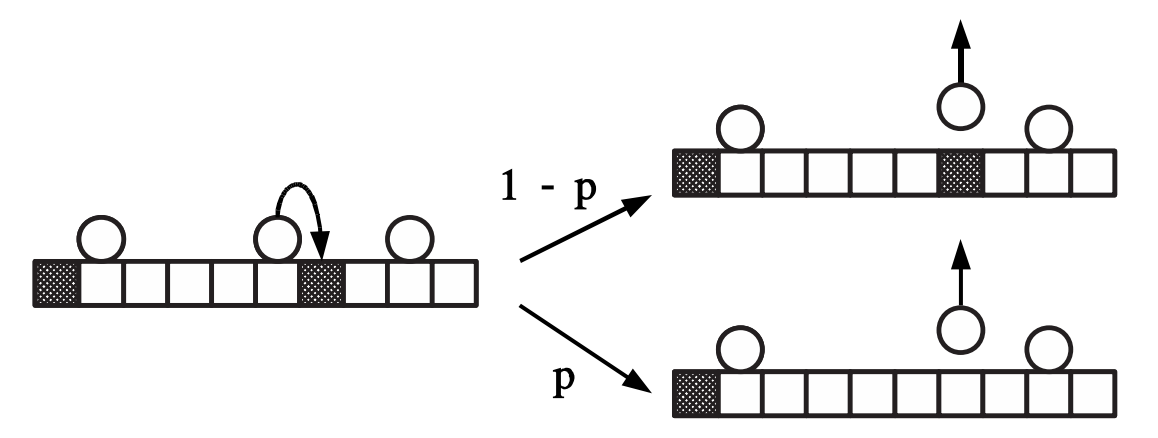
\includegraphics[width=\columnwidth]{./figures/031-EsquemaModelo.png}
  \captionof{figure}{Representação esquemática da dinâmica do modelo.
    Os sítios catalíticos (armadilhas) estão representados por quadrados pretos,
    enquanto sítios inativos, por quadrados brancos. Os círculos representam
    reagentes que difundem pela rede. Quando um reagente se desloca para uma
    armadilha, deixa o sistema instantaneamente. Quando este evento ocorre, com
    probabilidade \textit{p}, o sítio perde sua atividade catalítica e passa a
    ser um sítio inativo (\ref{Equation-032-ModeloEnvenenamento}). Com probabilidade 1 -
    \textit{p}, o sítio matém sua condição de sítio catalítico
    (\ref{Equation-031-ModeloTradicional}) \cite{3}.}
	\label{Figure-031-EsquemaModelo}
}
